\documentclass[12pt]{article}
\usepackage[papersize={20cm,30cm},tmargin=5mm,bmargin=5mm,lmargin=5mm,rmargin=5mm]{geometry}
\usepackage{tikz-network}


\definecolor{RosaMexicano}{RGB}{245, 0, 135}
\definecolor{Azul}{RGB}{0, 0, 255}
\definecolor{VerdeOlivo}{RGB}{172, 152, 60}
\definecolor{Verde}{RGB}{5, 135, 65}
\definecolor{Gris}{RGB}{170, 170, 170}

\begin{document}
\pagestyle{empty}
\thispagestyle{empty}
    \section{Grafo sin peso y matriz de adyacencia}
    \begin{figure}[h]
        \centering
        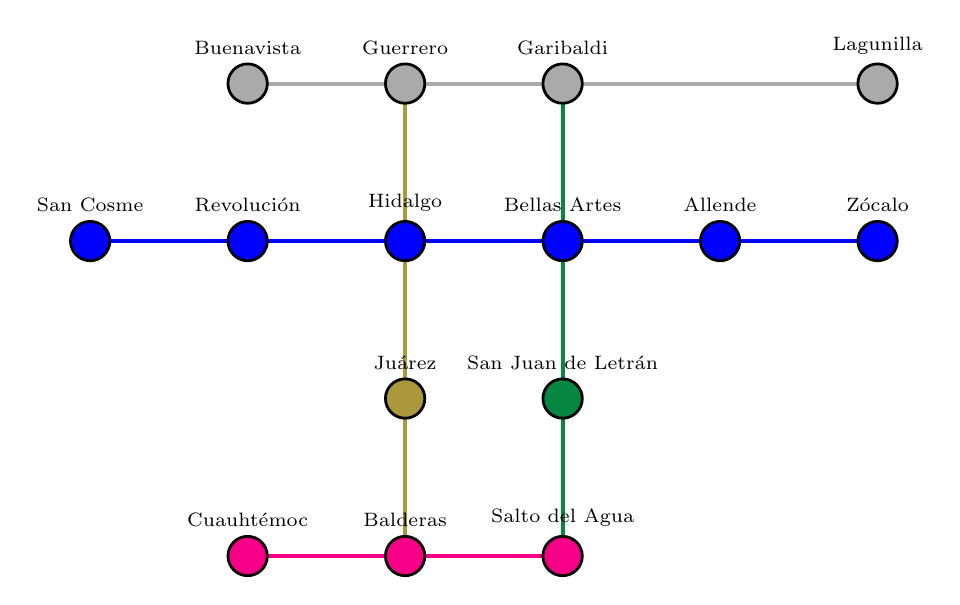
\begin{tikzpicture}
            %Malla 6 x 4
            \Vertex[x=-3,y=3,size=0.5, label=Buenavista,position=above, color=Gris]{A}
            \Vertex[x=-1,y=3,size=0.5, label=Guerrero,position=above, color=Gris]{B}
            \Vertex[x=1,y=3,size=0.5, label=Garibaldi,position=above, color=Gris]{C}
            \Vertex[x=5,y=3,size=0.5, label=Lagunilla,position=above, color=Gris]{D}
            \Edge[color=Gris](A)(B)
            \Edge[color=Gris](B)(C)
            \Edge[color=Gris](C)(D)
            \Vertex[x=-5,y=1,size=0.5, label=San Cosme,position=above, color=Azul]{E}
            \Vertex[x=-3,y=1,size=0.5, label=Revolución,position=above, color=Azul]{F}
            \Vertex[x=-1,y=1,size=0.5, label=Hidalgo,position=above, color=Azul]{G}
            \Vertex[x=1,y=1,size=0.5, label=Bellas Artes,position=above, color=Azul]{H}
            \Vertex[x=3,y=1,size=0.5, label=Allende,position=above, color=Azul]{I}
            \Vertex[x=5,y=1,size=0.5, label=Zócalo,position=above, color=Azul]{J}
            \Edge[color=Azul](E)(F)
            \Edge[color=Azul](F)(G)
            \Edge[color=Azul](G)(H)
            \Edge[color=Azul](H)(I)
            \Edge[color=Azul](I)(J)
            \Edge[color=VerdeOlivo](B)(G)
            \Edge[color=Verde](C)(H)
            \Vertex[x=-1,y=-1,size=0.5, label=Juárez,position=above, color=VerdeOlivo]{K}
            \Vertex[x=1,y=-1,size=0.5, label=San Juan de Letrán,position=above, color=Verde]{L}
            \Edge[color=VerdeOlivo](K)(G)
            \Edge[color=Verde](L)(H)
            \Vertex[x=-3,y=-3,size=0.5, label=Cuauhtémoc,position=above, color=RosaMexicano]{M}
            \Vertex[x=-1,y=-3,size=0.5, label=Balderas,position=above, color=RosaMexicano]{N}
            \Vertex[x=1,y=-3,size=0.5, label=Salto del Agua,position=above, color=RosaMexicano]{O}
            \Edge[color=RosaMexicano](M)(N)
            \Edge[color=RosaMexicano](N)(O)
            \Edge[color=VerdeOlivo](K)(N)
            \Edge[color=Verde](L)(O)
        \end{tikzpicture}
    \end{figure}
    \[
        \left[
            \begin{array}{*{15}c}
                0 & 1 & 0 & 0 & 0 & 0 & 0 & 0 & 0 & 0 & 0 & 0 & 0 & 0 & 0 \\
                1 & 0 & 1 & 0 & 0 & 0 & 1 & 0 & 0 & 0 & 0 & 0 & 0 & 0 & 0 \\
                0 & 1 & 0 & 1 & 0 & 0 & 0 & 1 & 0 & 0 & 0 & 0 & 0 & 0 & 0 \\
                0 & 0 & 1 & 0 & 0 & 0 & 0 & 0 & 0 & 0 & 0 & 0 & 0 & 0 & 0 \\
                0 & 0 & 0 & 0 & 0 & 1 & 0 & 0 & 0 & 0 & 0 & 0 & 0 & 0 & 0 \\
                0 & 0 & 0 & 0 & 1 & 0 & 1 & 0 & 0 & 0 & 0 & 0 & 0 & 0 & 0 \\
                0 & 1 & 0 & 0 & 0 & 1 & 0 & 1 & 0 & 0 & 1 & 0 & 0 & 0 & 0 \\
                0 & 0 & 1 & 0 & 0 & 0 & 1 & 0 & 1 & 0 & 0 & 1 & 0 & 0 & 0 \\
                0 & 0 & 0 & 0 & 0 & 0 & 0 & 1 & 0 & 1 & 0 & 0 & 0 & 0 & 0 \\
                0 & 0 & 0 & 0 & 0 & 0 & 0 & 0 & 1 & 0 & 0 & 0 & 0 & 0 & 0 \\
                0 & 0 & 0 & 0 & 0 & 0 & 1 & 0 & 0 & 0 & 0 & 0 & 0 & 1 & 0 \\
                0 & 0 & 0 & 0 & 0 & 0 & 0 & 1 & 0 & 0 & 0 & 0 & 0 & 0 & 1 \\
                0 & 0 & 0 & 0 & 0 & 0 & 0 & 0 & 0 & 0 & 0 & 0 & 0 & 1 & 0 \\
                0 & 0 & 0 & 0 & 0 & 0 & 0 & 0 & 0 & 0 & 1 & 0 & 1 & 0 & 1 \\
                0 & 0 & 0 & 0 & 0 & 0 & 0 & 0 & 0 & 0 & 0 & 1 & 0 & 1 & 0 \\
            \end{array}
        \right]
    \]
    \newpage
    \section{Grafo y matriz de adyacencia con peso}
    \begin{figure}
        \centering
        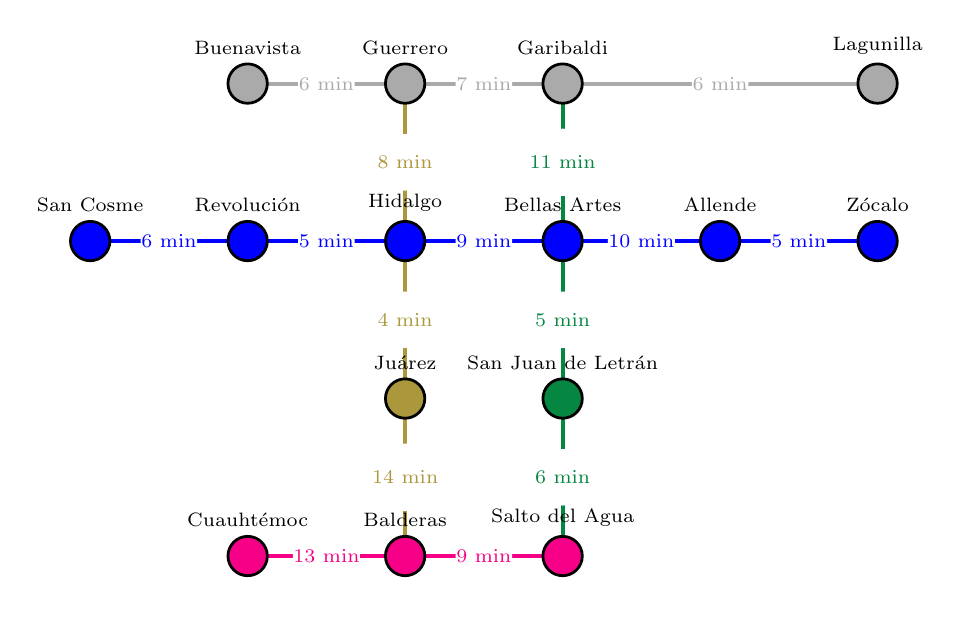
\begin{tikzpicture}
            %Malla 6 x 4
            \Vertex[x=-3,y=3,size=0.5, label=Buenavista,position=above, color=Gris]{A}
            \Vertex[x=-1,y=3,size=0.5, label=Guerrero,position=above, color=Gris]{B}
            \Vertex[x=1,y=3,size=0.5, label=Garibaldi,position=above, color=Gris]{C}
            \Vertex[x=5,y=3,size=0.5, label=Lagunilla,position=above, color=Gris]{D}
            \Edge[color=Gris, label=6 min](A)(B)
            \Edge[color=Gris, label=7 min](B)(C)
            \Edge[color=Gris, label=6 min](C)(D)
            \Vertex[x=-5,y=1,size=0.5, label=San Cosme,position=above, color=Azul]{E}
            \Vertex[x=-3,y=1,size=0.5, label=Revolución,position=above, color=Azul]{F}
            \Vertex[x=-1,y=1,size=0.5, label=Hidalgo,position=above, color=Azul]{G}
            \Vertex[x=1,y=1,size=0.5, label=Bellas Artes,position=above, color=Azul]{H}
            \Vertex[x=3,y=1,size=0.5, label=Allende,position=above, color=Azul]{I}
            \Vertex[x=5,y=1,size=0.5, label=Zócalo,position=above, color=Azul]{J}
            \Edge[color=Azul, label=6 min](E)(F)
            \Edge[color=Azul, label=5 min](F)(G)
            \Edge[color=Azul, label=9 min](G)(H)
            \Edge[color=Azul, label=10 min](H)(I)
            \Edge[color=Azul, label=5 min](I)(J)
            \Edge[color=VerdeOlivo, label=8 min](B)(G)
            \Edge[color=Verde, label=11 min](C)(H)
            \Vertex[x=-1,y=-1,size=0.5, label=Juárez,position=above, color=VerdeOlivo]{K}
            \Vertex[x=1,y=-1,size=0.5, label=San Juan de Letrán,position=above, color=Verde]{L}
            \Edge[color=VerdeOlivo, label=4 min](K)(G)
            \Edge[color=Verde, label=5 min](L)(H)
            \Vertex[x=-3,y=-3,size=0.5, label=Cuauhtémoc,position=above, color=RosaMexicano]{M}
            \Vertex[x=-1,y=-3,size=0.5, label=Balderas,position=above, color=RosaMexicano]{N}
            \Vertex[x=1,y=-3,size=0.5, label=Salto del Agua,position=above, color=RosaMexicano]{O}
            \Edge[color=RosaMexicano, label=13 min](M)(N)
            \Edge[color=RosaMexicano, label=9 min](N)(O)
            \Edge[color=VerdeOlivo, label=14 min](K)(N)
            \Edge[color=Verde, label=6 min](L)(O)
        \end{tikzpicture}
    \end{figure}
    \[
        \left[
            \begin{array}{*{15}c}
                0 & 6 & 0 & 0 & 0 & 0 & 0 & 0 & 0 & 0 & 0 & 0 & 0 & 0 & 0 \\
                6 & 0 & 7 & 0 & 0 & 0 & 8 & 0 & 0 & 0 & 0 & 0 & 0 & 0 & 0 \\
                0 & 7 & 0 & 6 & 0 & 0 & 0 & 11 & 0 & 0 & 0 & 0 & 0 & 0 & 0 \\
                0 & 0 & 6 & 0 & 0 & 0 & 0 & 0 & 0 & 0 & 0 & 0 & 0 & 0 & 0 \\
                0 & 0 & 0 & 0 & 0 & 6 & 0 & 0 & 0 & 0 & 0 & 0 & 0 & 0 & 0 \\
                0 & 0 & 0 & 0 & 6 & 0 & 5 & 0 & 0 & 0 & 0 & 0 & 0 & 0 & 0 \\
                0 & 8 & 0 & 0 & 0 & 5 & 0 & 9 & 0 & 0 & 4 & 0 & 0 & 0 & 0 \\
                0 & 0 & 11 & 0 & 0 & 0 & 9 & 0 & 10 & 0 & 0 & 5 & 0 & 0 & 0 \\
                0 & 0 & 0 & 0 & 0 & 0 & 0 & 10 & 0 & 5 & 0 & 0 & 0 & 0 & 0 \\
                0 & 0 & 0 & 0 & 0 & 0 & 0 & 0 & 5 & 0 & 0 & 0 & 0 & 0 & 0 \\
                0 & 0 & 0 & 0 & 0 & 0 & 4 & 0 & 0 & 0 & 0 & 0 & 0 & 14 & 0 \\
                0 & 0 & 0 & 0 & 0 & 0 & 0 & 5 & 0 & 0 & 0 & 0 & 0 & 0 & 6 \\
                0 & 0 & 0 & 0 & 0 & 0 & 0 & 0 & 0 & 0 & 0 & 0 & 0 & 13 & 0 \\
                0 & 0 & 0 & 0 & 0 & 0 & 0 & 0 & 0 & 0 & 14 & 0 & 13 & 0 & 9 \\
                0 & 0 & 0 & 0 & 0 & 0 & 0 & 0 & 0 & 0 & 0 & 6 & 0 & 9 & 0 \\
            \end{array}
        \right]
    \]
    \newpage
    \section{Grafo y matriz de adyacencia (conveniente) con peso}
    \begin{figure}
        \centering
        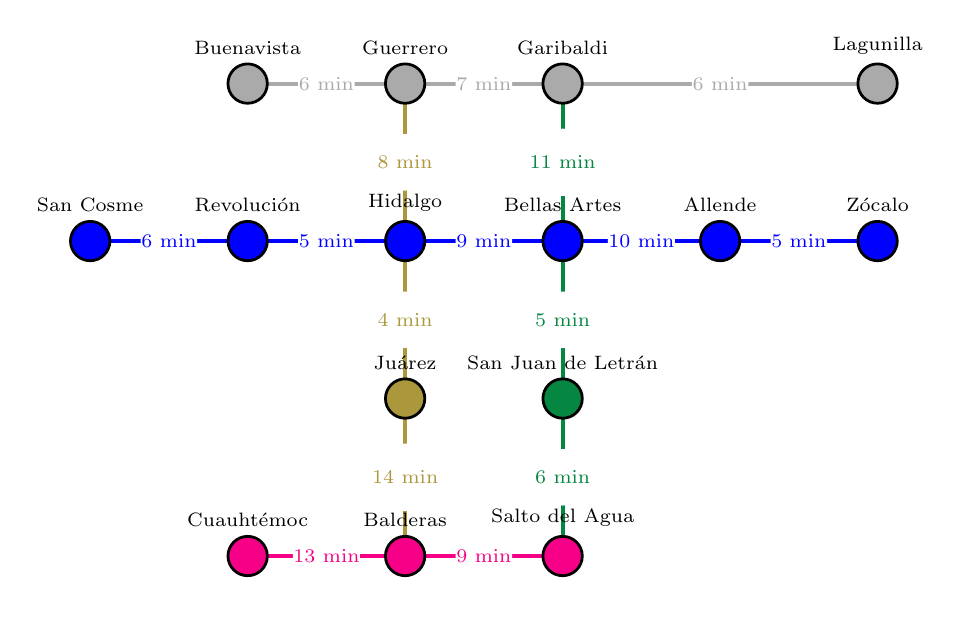
\begin{tikzpicture}
            %Malla 6 x 4
            \Vertex[x=-3,y=3,size=0.5, label=Buenavista,position=above, color=Gris]{A}
            \Vertex[x=-1,y=3,size=0.5, label=Guerrero,position=above, color=Gris]{B}
            \Vertex[x=1,y=3,size=0.5, label=Garibaldi,position=above, color=Gris]{C}
            \Vertex[x=5,y=3,size=0.5, label=Lagunilla,position=above, color=Gris]{D}
            \Edge[color=Gris, label=6 min](A)(B)
            \Edge[color=Gris, label=7 min](B)(C)
            \Edge[color=Gris, label=6 min](C)(D)
            \Vertex[x=-5,y=1,size=0.5, label=San Cosme,position=above, color=Azul]{E}
            \Vertex[x=-3,y=1,size=0.5, label=Revolución,position=above, color=Azul]{F}
            \Vertex[x=-1,y=1,size=0.5, label=Hidalgo,position=above, color=Azul]{G}
            \Vertex[x=1,y=1,size=0.5, label=Bellas Artes,position=above, color=Azul]{H}
            \Vertex[x=3,y=1,size=0.5, label=Allende,position=above, color=Azul]{I}
            \Vertex[x=5,y=1,size=0.5, label=Zócalo,position=above, color=Azul]{J}
            \Edge[color=Azul, label=6 min](E)(F)
            \Edge[color=Azul, label=5 min](F)(G)
            \Edge[color=Azul, label=9 min](G)(H)
            \Edge[color=Azul, label=10 min](H)(I)
            \Edge[color=Azul, label=5 min](I)(J)
            \Edge[color=VerdeOlivo, label=8 min](B)(G)
            \Edge[color=Verde, label=11 min](C)(H)
            \Vertex[x=-1,y=-1,size=0.5, label=Juárez,position=above, color=VerdeOlivo]{K}
            \Vertex[x=1,y=-1,size=0.5, label=San Juan de Letrán,position=above, color=Verde]{L}
            \Edge[color=VerdeOlivo, label=4 min](K)(G)
            \Edge[color=Verde, label=5 min](L)(H)
            \Vertex[x=-3,y=-3,size=0.5, label=Cuauhtémoc,position=above, color=RosaMexicano]{M}
            \Vertex[x=-1,y=-3,size=0.5, label=Balderas,position=above, color=RosaMexicano]{N}
            \Vertex[x=1,y=-3,size=0.5, label=Salto del Agua,position=above, color=RosaMexicano]{O}
            \Edge[color=RosaMexicano, label=13 min](M)(N)
            \Edge[color=RosaMexicano, label=9 min](N)(O)
            \Edge[color=VerdeOlivo, label=14 min](K)(N)
            \Edge[color=Verde, label=6 min](L)(O)
        \end{tikzpicture}
    \end{figure}
    \[
        \left[
            \begin{array}{*{15}c}
                -1 & 6 & -1 & -1 & -1 & -1 & -1 & -1 & -1 & -1 & -1 & -1 & -1 & -1 & -1 \\
                6 & -1 & 7 & -1 & -1 & -1 & 8 & -1 & -1 & -1 & -1 & -1 & -1 & -1 & -1 \\
                -1 & 7 & -1 & 6 & -1 & -1 & -1 & 11 & -1 & -1 & -1 & -1 & -1 & -1 & -1 \\
                -1 & -1 & 6 & -1 & -1 & -1 & -1 & -1 & -1 & -1 & -1 & -1 & -1 & -1 & -1 \\
                -1 & -1 & -1 & -1 & -1 & 6 & -1 & -1 & -1 & -1 & -1 & -1 & -1 & -1 & -1 \\
                -1 & -1 & -1 & -1 & 6 & -1 & 5 & -1 & -1 & -1 & -1 & -1 & -1 & -1 & -1 \\
                -1 & 8 & -1 & -1 & -1 & 5 & -1 & 9 & -1 & -1 & 4 & -1 & -1 & -1 & -1 \\
                -1 & -1 & 11 & -1 & -1 & -1 & 9 & -1 & 10 & -1 & -1 & -1 & -1 & -1 & -1 \\
                -1 & -1 & -1 & -1 & -1 & -1 & -1 & 10 & -1 & 5 & -1 & -1 & -1 & -1 & -1 \\
                -1 & -1 & -1 & -1 & -1 & -1 & -1 & -1 & 5 & -1 & -1 & -1 & -1 & -1 & -1 \\
                -1 & -1 & -1 & -1 & -1 & -1 & 4 & -1 & -1 & -1 & -1 & -1 & -1 & 14 & -1 \\
                -1 & -1 & -1 & -1 & -1 & -1 & -1 & 5 & -1 & -1 & -1 & -1 & -1 & -1 & 6 \\
                -1 & -1 & -1 & -1 & -1 & -1 & -1 & -1 & -1 & -1 & -1 & -1 & -1 & 13 & -1 \\
                -1 & -1 & -1 & -1 & -1 & -1 & -1 & -1 & -1 & -1 & 14 & -1 & 13 & -1 & 9 \\
                -1 & -1 & -1 & -1 & -1 & -1 & -1 & -1 & -1 & -1 & -1 & 6 & -1 & 9 & -1 \\
            \end{array}
        \right]
    \]
\end{document}